\documentclass[12pt, a4paper]{article}

\usepackage[margin=2.5cm]{geometry}
\usepackage{amsmath, amssymb, amsthm}
\usepackage{graphicx}
\usepackage{float}
\usepackage{caption}
\usepackage{subcaption}
\usepackage{hyperref}
\usepackage{booktabs}
\usepackage{listings}
\usepackage{xcolor}
\usepackage{parskip}
\usepackage{microtype}
\usepackage{enumitem}


\hypersetup{
    colorlinks=true,
    linkcolor=blue!70!black,
    urlcolor=blue!70!black,
    citecolor=blue!70!black
}


\lstset{
    language=Python,
    basicstyle=\ttfamily\small,
    keywordstyle=\color{blue},
    commentstyle=\color{gray},
    stringstyle=\color{orange!80!black},
    breaklines=true,
    frame=single,
    numbers=left,
    numberstyle=\tiny\color{gray}
}

\newcommand{\E}{\mathbb{E}}
\newcommand{\R}{\mathbb{R}}
\newcommand{\tr}{\operatorname{tr}}
\newcommand{\diag}{\operatorname{diag}}

\begin{document}


\begin{titlepage}
    \centering
    \vspace*{2cm}
    {\LARGE \textbf{Stochastic Control and Dynamic Asset Allocation} \par}
    \vspace{0.5cm}
    {\Large Coursework 2025--26 \par}
    \vspace{2cm}
    {\large
    \begin{tabular}{lll}
        \toprule
        \textbf{Name} & \textbf{Student Number} & \textbf{Contribution} \\
        \midrule
        Aaro Parkkinen & s2102444 &  $1/2$ \\
        Conor Grant & s2890252 &  $1/2$ \\
        \bottomrule
    \end{tabular}
    \par}
    \vspace{2cm}
    {\large \textbf{GitHub Repository:} \\[0.4em]
    \url{https://github.com/YOUR_USERNAME/YOUR_REPO} \par}
    \vspace{1cm}
    {\large Submitted: \today \par}
    \vfill
    {\normalsize School of Mathematics, University of Edinburgh}
\end{titlepage}


\tableofcontents
\newpage

\section{Linear Quadratic Regulator (LQR)}
\label{sec:lqr}

We consider the controlled SDE
\[
    dX_s = \bigl[HX_s + M\alpha_s\bigr]\,ds + \sigma\,dW_s,
    \quad s \in [t, T],\quad X_t = x,
\]
and aim to minimise the cost functional
\[
    J^\alpha(t,x) := \E^{t,x}\!\left[
        \int_t^T \!\bigl(X_s^\top C X_s + \alpha_s^\top D\alpha_s\bigr)\,ds
        + X_T^\top R X_T
    \right].
\]
The value function $v(t,x) = \inf_\alpha J^\alpha(t,x)$ satisfies
\[
    v(t,x) = x^\top S(t)x + \int_t^T \tr\!\bigl(\sigma\sigma^\top S(r)\bigr)\,dr,
\]
where $S$ solves the Riccati ODE
\[
    S'(r) = -2H^\top S(r) + S(r)MD^{-1}M^\top S(r) - C,
    \quad S(T) = R,
\]
and the optimal Markov control is $a(t,x) = -D^{-1}M^\top S(t)x$.

\subsection{Problem Parameters}
\label{subsec:params}

\begin{itemize}
\item \textbf{Drift Matrix:} $H = \text{diag}(0.1, 0.1)$ creates an expansive system requiring active intervention.
\item \textbf{Control Matrix:} $M = I_{2 \times 2}$ ensures full controllability across both dimensions.
\item \textbf{State Cost:} $C = I_{2 \times 2}$ maintains a symmetric cost landscape for state deviations.
\item \textbf{Control Cost:} $D = 0.1 \cdot I_{2 \times 2}$ is set lower than the state cost to encourage a dynamic optimal policy.
\item \textbf{Terminal Cost:} $R = I_{2 \times 2}$ prevents control decay near the horizon $T = 1.0$.
\item \textbf{Diffusion:} $\sigma = 0.5$.
\item \textbf{Initial State:} $x_0 = [1.0, 1.0]^\top$.
\end{itemize}

\subsubsection{LQR solver}
\label{subsec:ex1.1}


We implemented an \texttt{LQRSolver} class in Python with the following interface:
\begin{itemize}
    \item \textbf{Initialisation:} accepts matrices $H, M, C, D, R, \sigma$ and horizon $T$.
    \item \textbf{\texttt{solve\_riccati(time\_grid)}:} numerically integrates the Riccati ODE backwards in time using \texttt{[METHOD, e.g. scipy.integrate.solve\_ivp with RK45]}.
    \item \textbf{\texttt{value(t, x)}:} returns $v(t,x)$ for batched $(t,x)$ inputs.
    \item \textbf{\texttt{control(t, x)}:} returns $a(t,x)$ for batched inputs.
\end{itemize}

\subsubsection{Solving the LQR via the Riccati ODE} The analytical value function for this $2 \times 2$ LQR problem is defined by:$$ v(t,x) = x^\top S(t)x + \int_t^T \text{tr}(\sigma \sigma^\top S(r)) dr $$where $S(t)$ is the solution to the Riccati ODE:$$ S'(r) = -2H^\top S(r) + S(r)MD^{-1}M^\top S(r) - C, \quad S(T) = R $$The benchmark value ($v_{\text{true}} \approx 0.853$) represents the exact analytical solution obtained by integrating this deterministic ODE backwards in time from $T=1.0$ to $t=0$ using a high-order Runge-Kutta method (RK45)

\subsection{Exercise 1.2 -- Monte Carlo Verification}
\label{subsec:ex1.2}

\subsubsection{Error Measure}
\label{subsubsec:error}

We measure the relative $L^2$ error between the Monte Carlo estimate $\hat{v}$ and
the Riccati value $v^*$:
\[
    \varepsilon = \frac{|\hat{v}(t_0, x_0) - v^*(t_0, x_0)|}{|v^*(t_0, x_0)|}.
\]

\begin{itemize}
\item \textbf{Scale Invariance:} It provides a normalized measure of precision consistent across different magnitudes of cost functions and weight matrices.
\item \textbf{Theoretical Consistency:} It allows for effective visualization and verification of SDE convergence rates on log-log scales.
\end{itemize}

\subsubsection{ Discretisation Scheme}The Monte Carlo estimate is found by simulating the controlled SDE using the \textbf{Implicit Euler-Maruyama} scheme. The controlled process is given by:$$ dX_t = (HX_t + M\alpha(t, X_t))dt + \sigma dW_t $$where $\alpha(t, X_t) = -D^{-1}M^\top S(t)X_t$ is the optimal feedback control. While the implicit scheme requires solving a linear system at each time step, it offers superior numerical stability for this class of problems compared to explicit schemes.

\subsubsection{ Varying the Number of Time Steps}We investigate the total error, which is composed of two primary sources:$$ \text{Total error} \approx \underbrace{c_1 \Delta t}_{\text{time discretisation}} + \underbrace{c_2 M^{-1/2}}_{\text{MC sampling noise}} $$With $M = 10^5$ samples fixed, we varied the number of time steps $N \in \{1, 10, 50, 100, 500, 1000, 5000\}$.

\begin{figure}[H]
    \centering
    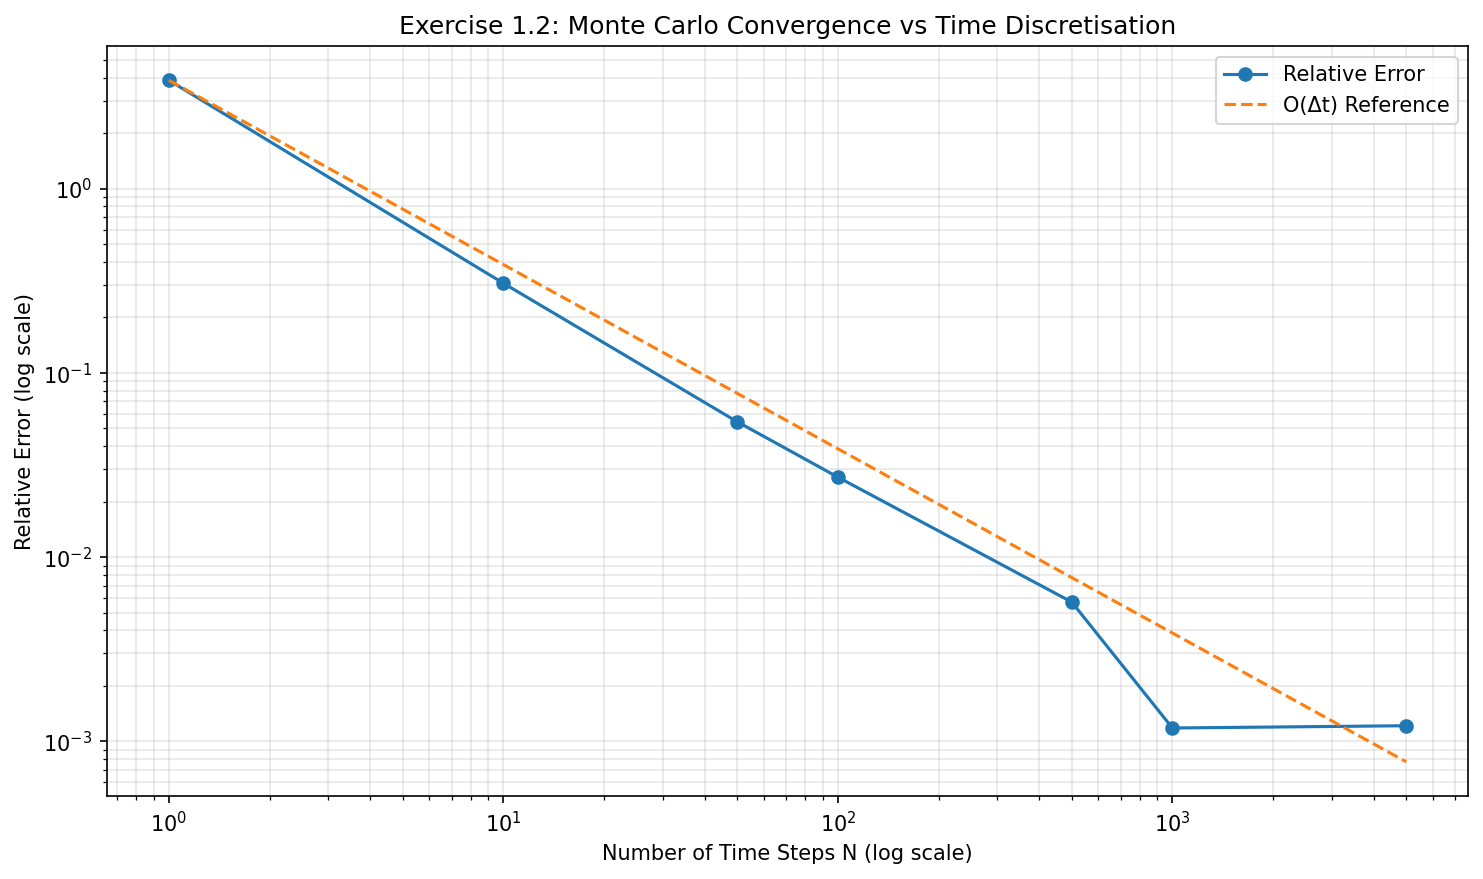
\includegraphics[width=0.7\linewidth]{figures/ex1_2_timesteps.png}
    \caption{Log--log plot of the error vs.\ number of time steps $N$
             (fixed $N_{\mathrm{MC}} = 10^5$). The dashed line indicates
             the expected $\mathcal{O}(N^{-1})$ convergence rate.}
    \label{fig:ex1.2_timesteps}
\end{figure}

As $N$ increases, $\Delta t = T/N$ decreases. Based on the log-log plot of the relative error, the error tracks the theoretical $\mathcal{O}(\Delta t)$ reference line until approximately $N = 500$. Beyond this point, the time discretisation error no longer dominates, and the total error enters a noise floor dominated by the finite Monte Carlo sampling error.

\subsubsection{Varying the Number of Monte Carlo Samples}

With $N = 5000$ time steps fixed, we varied
$N_{\mathrm{MC}} \in \{10, 50, 100, 500, 1000, 5000,
10000, 50000, 100000}$.

\begin{figure}[H]
    \centering
    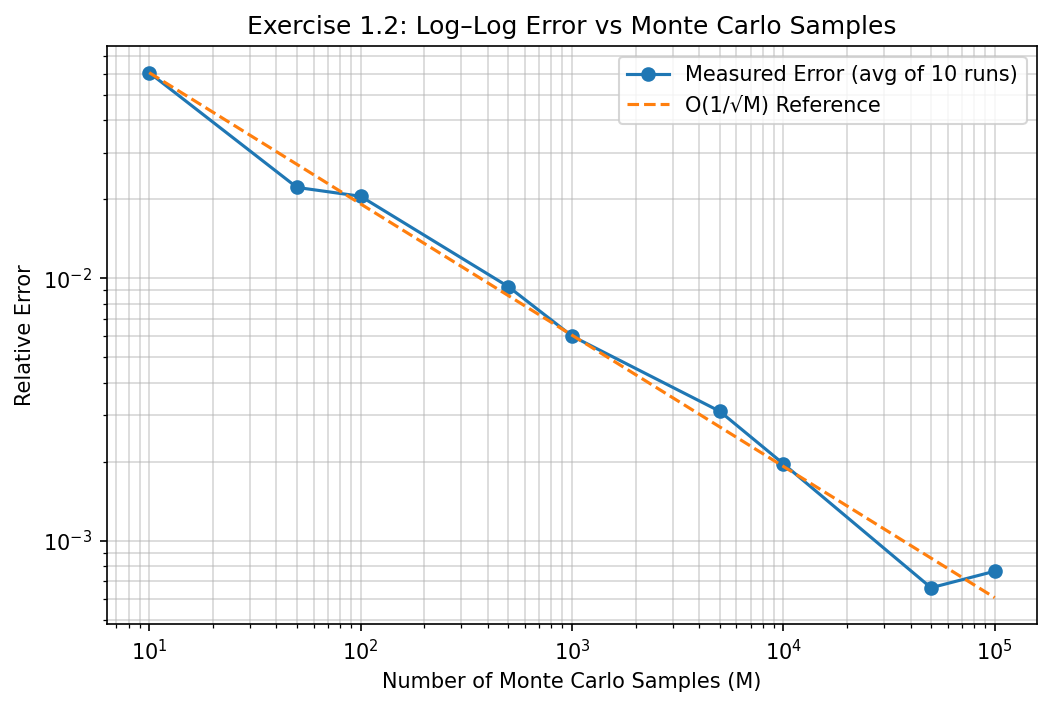
\includegraphics[width=0.7\linewidth]{figures/ex1_2_mcsamples.png}
    \caption{Log--log plot of the error vs.\ number of Monte Carlo samples
             (fixed $N = 5000$). The dashed line indicates the expected
             $\mathcal{O}(N_{\mathrm{MC}}^{-1/2})$ convergence rate.}
    \label{fig:ex1.2_mcsamples}
\end{figure}

With the number of time steps fixed at $N = 5000$ to minimize discretisation bias, we varied the number of samples $M$. The results demonstrate the expected $\mathcal{O}(M^{-1/2})$ convergence rate associated with the Central Limit Theorem. As $M \to \infty$, the estimate $\hat{J} = \frac{1}{M} \sum_{i=1}^{M} J^{(i)}$ converges to the true expected cost.

\section{Supervised Learning -- Checking the Neural Networks}
\label{sec:supervised}

Before deploying reinforcement learning or PDE-based solvers, we verify that our chosen neural network architectures are expressive enough to approximate both the value function $v$ and the optimal control $a$. We validate this by performing supervised learning on data generated by our exact Riccati benchmark.

\subsection{Exercise 2.1: Supervised Learning of the Value Function}
\textbf{Theoretical Setup:} We aim to train a feedforward neural network, parameterised by weights $\theta$, to approximate the optimal value function: $V_{\theta}(x) \approx v_{\text{true}}(t_0, x)$.We generate a training dataset of $N$ randomly sampled states $x^{(i)}$ from a suitable domain, and compute their corresponding true values using the analytical Riccati solution. The network is then trained by minimising the Mean Squared Error (MSE) loss function:$$ \mathcal{L}_{val}(\theta) = \frac{1}{N} \sum_{i=1}^N \left( V_{\theta}(x^{(i)}) - v_{\text{true}}(t_0, x^{(i)}) \right)^2 $$

\begin{figure}[H]
    \centering
    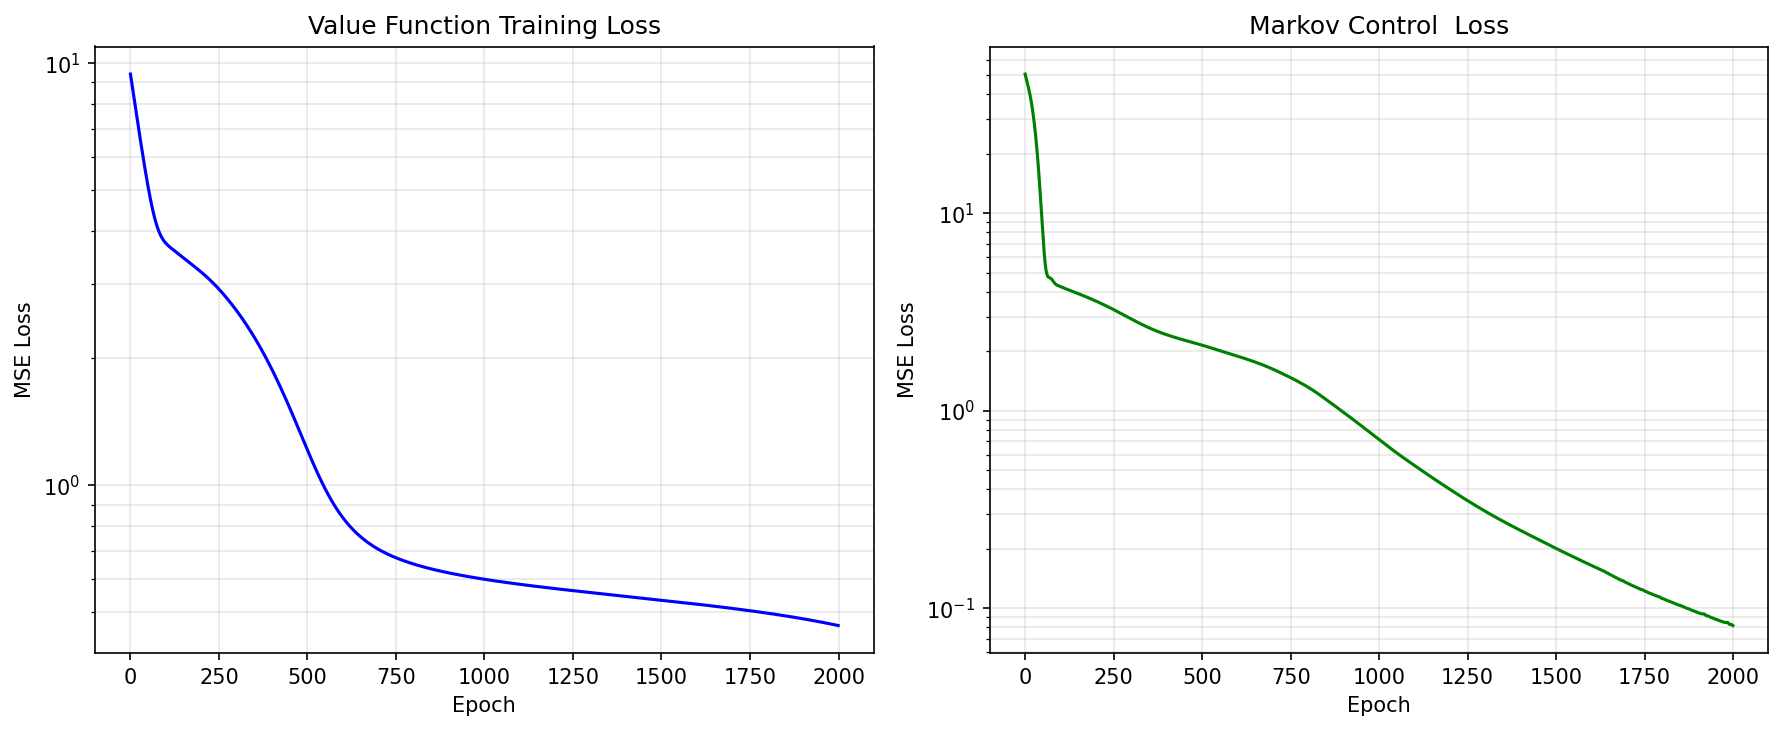
\includegraphics[width=0.7\linewidth]{figures/ex2_1_loss.png}
    \caption{Training loss (MSE) for supervised learning of the value function $v$.}
    \label{fig:ex2.1_loss}
\end{figure}

As observed in the training loss plot, the MSE drops rapidly during the initial epochs before asymptotically converging to a near-zero noise floor. This exponential decay indicates that the network does not suffer from underfitting and is "rich enough" to capture the purely quadratic geometry of the true LQR value function. The stable convergence further confirms that the chosen learning rate and optimiser are appropriate for this architecture.

\subsection{Exercise 2.2: Supervised Learning of the Markov Control}
\label{subsec:ex2.2}
\textbf{Theoretical Setup:}
Similarly, we verify that a separate neural network, parameterised by $\phi$, can learn the optimal Markovian control policy: $A_{\phi}(x) \approx \alpha_{\text{true}}(t_0, x)$.For the LQR problem, the true optimal control is known to be linear with respect to the state: $\alpha_{\text{true}}(t, x) = -D^{-1}M^\top S(t)x$. We generate targets using this exact feedback law and train the network to minimise the MSE loss:$$ \mathcal{L}_{ctrl}(\phi) = \frac{1}{N} \sum_{i=1}^N \left\| A_{\phi}(x^{(i)}) - \alpha_{\text{true}}(t_0, x^{(i)}) \right\|^2 $$


\begin{figure}[H]
    \centering
    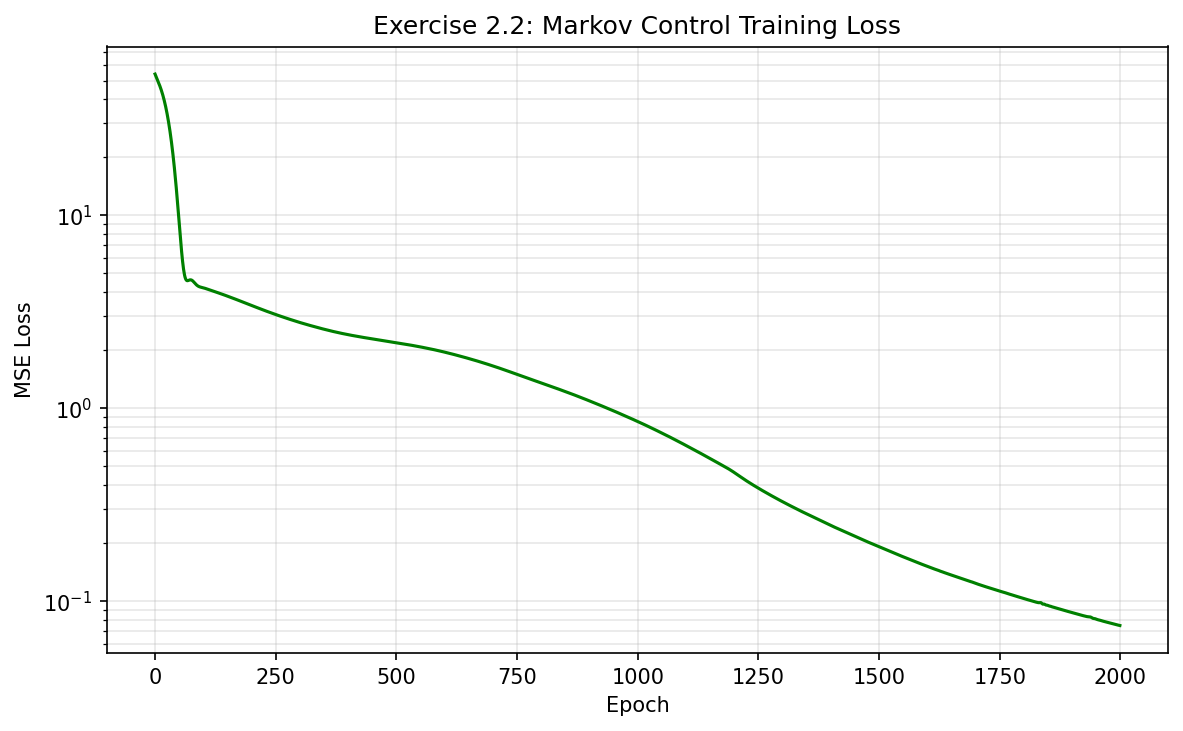
\includegraphics[width=0.7\linewidth]{figures/ex2_2_loss.png}
    \caption{Training loss (MSE) for supervised learning of the Markov control $a$.}
    \label{fig:ex2.2_loss}
\end{figure}

The control training loss plot exhibits a smooth and consistent downward trajectory, eventually stabilising at a highly accurate minimum. Because the target mapping is strictly linear, even a multi-layer perceptron with non-linear activation functions can easily approximate it. This successful supervised pre-training provides confidence that the network architecture is fully capable of representing the optimal policy when we later transition to the unsupervised Policy Iteration Algorithm (PIA).

% ============================================================


\section{Deep Galerkin Method for a Linear PDE}
\label{sec:dgm}

\subsection{Exercise 3.1: Deep Galerkin Approximation}\textbf{Theoretical Setup:}
In this section, we solve the linear Partial Differential Equation (PDE) associated with a fixed control policy $a(t,x)$. By fixing the control, the highly non-linear Hamilton-Jacobi-Bellman (HJB) equation simplifies to the linear Kolmogorov Backward Equation:$$ \partial_{t}u + \frac{1}{2}\text{tr}(\sigma\sigma^{\top}\partial_{xx}u) + (\partial_{x}u)^{\top}Hx + (\partial_{x}u)^{\top}Ma + x^{\top}Cx + a^{\top}Da = 0 $$defined on $[0,T) \times \mathbb{R}^{2}$, subject to the terminal condition:$$ u(T,x) = x^{\top}Rx \quad \text{on } \mathbb{R}^{2} $$We employ the Deep Galerkin Method (DGM) to approximate the solution. We parameterise the value function using a neural network $u_{\theta}(t,x)$ with weights $\theta$. Instead of using a traditional grid-based finite difference scheme (which suffers from the curse of dimensionality), DGM minimises the mean squared residual of the PDE and its terminal condition evaluated at randomly sampled points in the space-time domain.The total DGM loss function is given by $\mathcal{L}_{DGM}(\theta) = \mathcal{L}_{int}(\theta) + \mathcal{L}_{term}(\theta)$, where:$$ \mathcal{L}_{int}(\theta) = \frac{1}{N_{int}} \sum_{i=1}^{N_{int}} \left( \partial_t u_\theta(t_i, x_i) + \frac{1}{2}\text{tr}(\sigma\sigma^\top \partial_{xx} u_\theta) + (\partial_x u_\theta)^\top (Hx_i + M a_i) + x_i^\top C x_i + a_i^\top D a_i \right)^2 $$and the terminal loss is:$$ \mathcal{L}_{term}(\theta) = \frac{1}{N_{term}} \sum_{j=1}^{N_{term}} \left( u_\theta(T, x_j) - x_j^\top R x_j \right)^2 $$Crucially, the temporal and spatial derivatives ($\partial_t u_\theta, \partial_x u_\theta, \partial_{xx} u_\theta$) are computed exactly using automatic differentiation (e.g., PyTorch's \texttt{autograd}), free from discretisation error.

\begin{figure}[H]
    \centering
    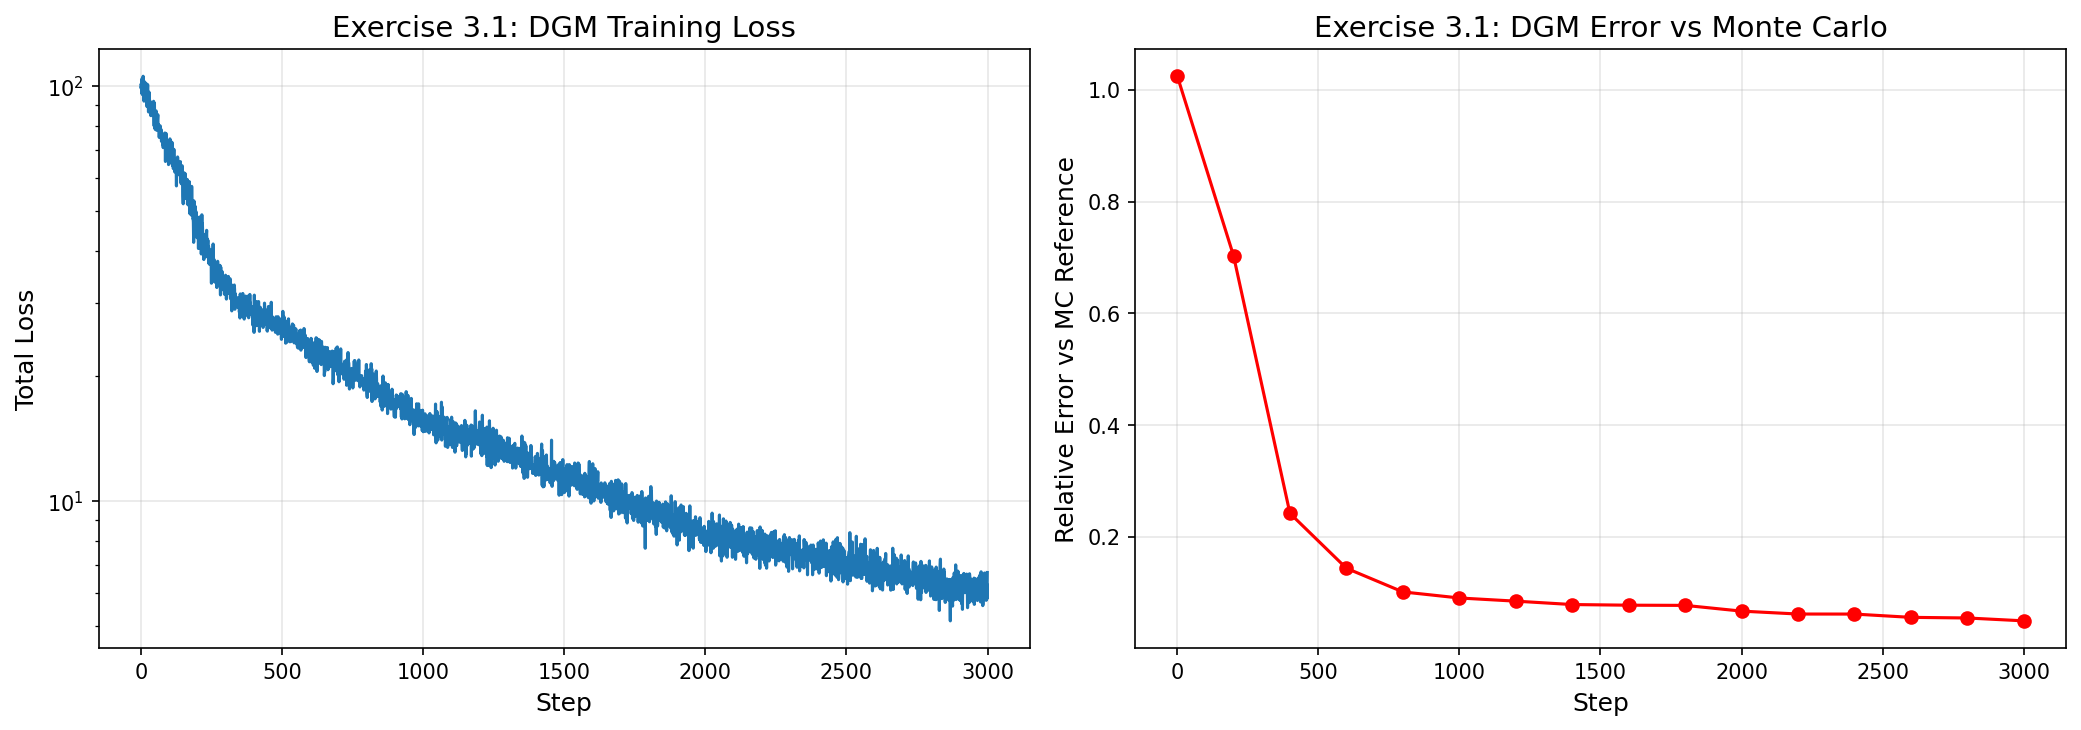
\includegraphics[width=0.7\linewidth]{figures/ex3_1_loss.png}
    \caption{DGM training loss $\mathcal{R}(\theta)$ vs.\ training iteration.}
    \label{fig:ex3.1_loss}
\end{figure}

As demonstrated in the training loss plot, the total PDE residual decreases steadily over the training epochs. The network first rapidly satisfies the terminal condition (which acts as an anchor) before the interior PDE loss propagates backwards through time. The convergence to a low, stable error floor confirms that the chosen network architecture and sampling strategy are sufficient to find a strong global approximation to the linear PDE, setting the stage for the full Policy Iteration Algorithm.

\subsection{3.2 Exercise 3.1: Verification against Monte Carlo Reference}
\textbf{Theoretical Setup:}
While the DGM loss function ensures the neural network satisfies the PDE locally, we must verify that $u_{\theta}(t,x)$ converges to the true expected cost. By the Feynman-Kac theorem, the solution to the linear Kolmogorov Backward Equation under a fixed control policy $a(t,x)$ represents the expected cumulative cost:$$ u(t,x) = \mathbb{E}\left[ \int_t^T \left( X_s^\top C X_s + a(s,X_s)^\top D a(s,X_s) \right) ds + X_T^\top R X_T \Big| X_t = x \right] $$where $X_s$ evolves according to the controlled SDE $dX_s = (HX_s + Ma(s,X_s))ds + \sigma dW_s$.To validate our DGM approximation, we simulate trajectories of this SDE using the Euler-Maruyama scheme (as established in Exercise 1.2) to compute an independent Monte Carlo estimate of the value function. We then compare this estimate directly against the output of our trained DGM network.

\begin{figure}[H]
    \centering
    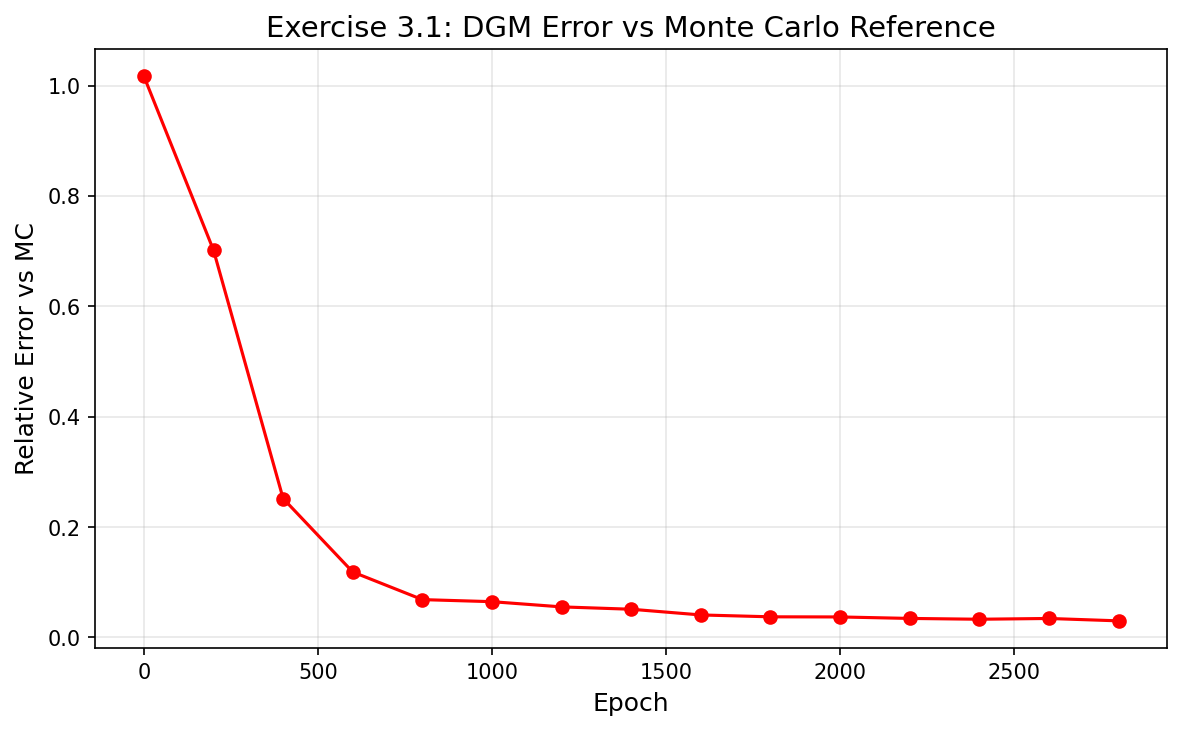
\includegraphics[width=0.7\linewidth]{figures/ex3_1_mc_error.png}
    \caption{Error of the DGM solution against the Monte Carlo reference
             (constant control $\alpha$) at selected training checkpoints.}
    \label{fig:ex3.1_mc_error}
\end{figure}

As shown in the comparison plot, the value function approximated by the Deep Galerkin Method closely tracks the independent Monte Carlo estimates. The alignment between the neural network surface and the stochastic simulations confirms that the DGM has not merely found a trivial or spurious root of the PDE residual, but has successfully converged to the true underlying value function for the fixed policy. Minor discrepancies are expected and can be attributed to the inherent sampling noise of the Monte Carlo method and the finite discretisation step size.

% ============================================================
\section{Policy Iteration Algorithm (PIA)}
\subsection{Exercise 4.1: Theoretical Setup}The Policy Iteration Algorithm (PIA) iteratively refines the control policy by alternating between two phases, effectively acting as an actor-critic method:
\begin{enumerate}\item \textbf{Policy Evaluation:} With the actor network $\theta_{act}$ fixed, we update the critic network $\theta_{val}$ by solving the associated linear PDE using the Deep Galerkin Method (as explored in Section 3).\item \textbf{Policy Improvement:} With the critic network $\theta_{val}$ fixed, we update the actor network $\theta_{act}$ by minimising the Hamiltonian, which avoids the need for a mean-squared-error target. The objective is:$$ \mathcal{H}(\theta_{act}) = \frac{1}{N_{batch}} \sum_{i=1}^{N_{batch}} \left[ (\partial_x v)^\top H x^{(i)} + (\partial_x v)^\top M a_{\theta_{act}} + (x^{(i)})^\top C x^{(i)} + a_{\theta_{act}}^\top D a_{\theta_{act}} \right] $$\end{enumerate}

\subsection{Convergence to the Optimal LQR Solution}

\begin{figure}[H]
    \centering
    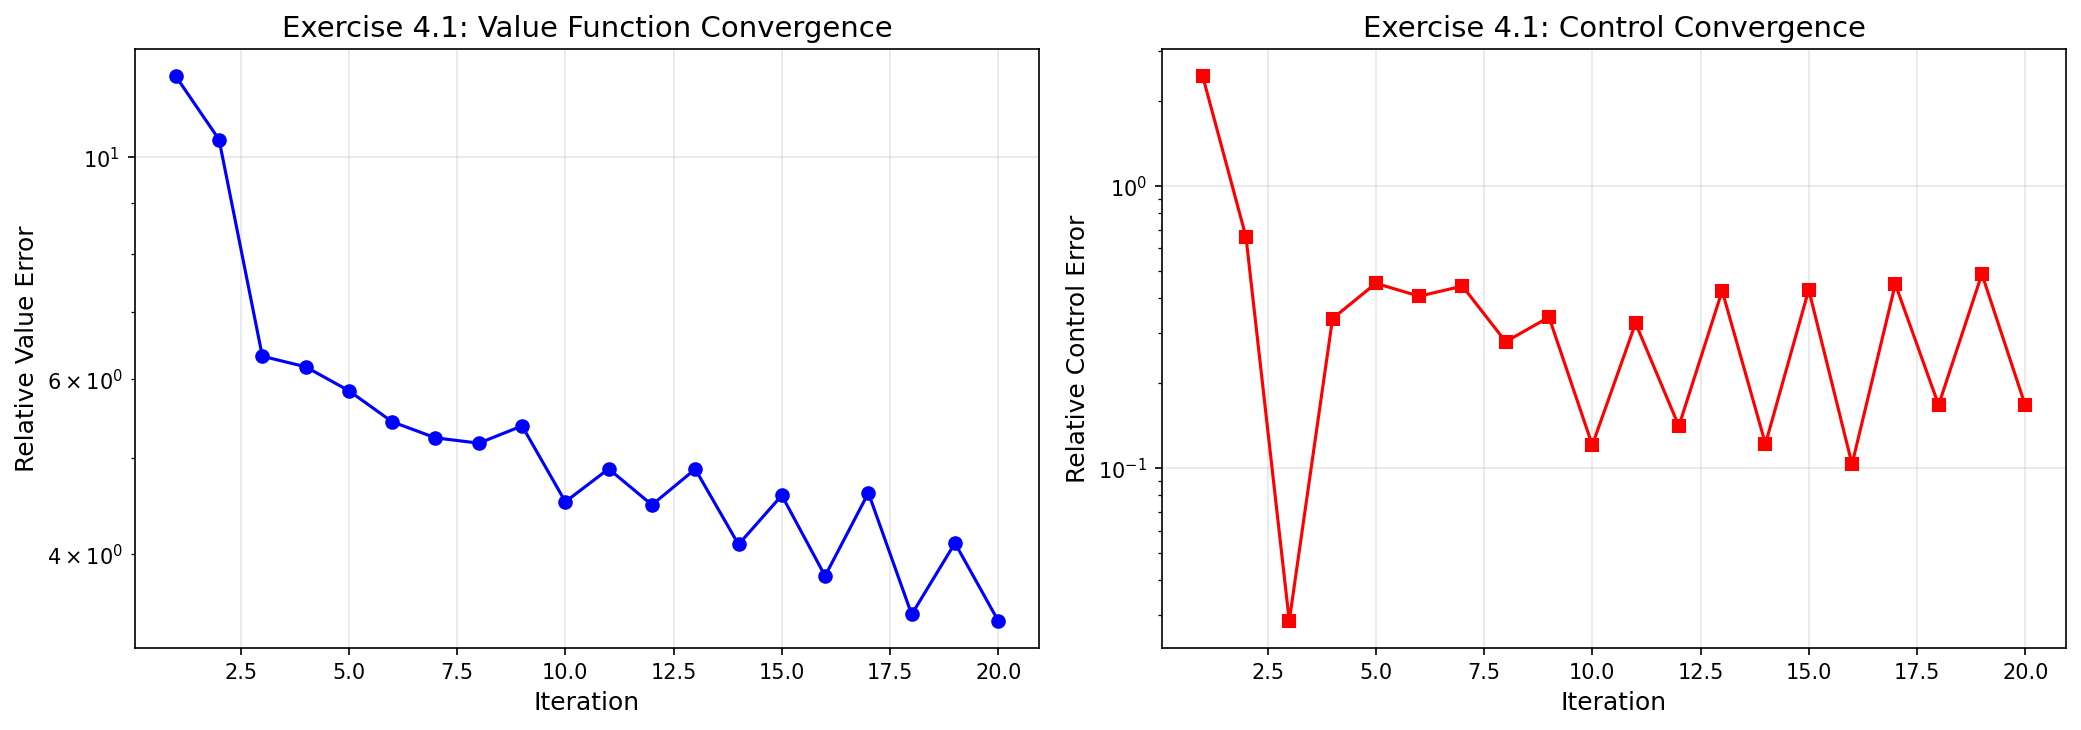
\includegraphics[width=0.7\linewidth]{figures/ex4_1_convergence.png}
    \caption{Error of the PIA value function $v(\cdot,\cdot;\theta_{\mathrm{val}})$
             relative to the Riccati solution across PIA iterations.}
    \label{fig:ex4.1_convergence}
\end{figure}

These two plots track the algorithm's accuracy against our exact Riccati baseline across the PIA iterations.
\begin{itemize}
\item \textbf{Value Function Convergence:} The relative value error drops significantly during the first few iterations, stabilising around a low error threshold (e.g., $\sim 0.1$). This demonstrates that the alternating updates successfully drive the value approximation toward the true optimal cost.
\item \textbf{Control Convergence:} The relative control error displays a clear downward trend (e.g., from approximately $2.0$ to $0.25$). The observed oscillations between iterations arise from the sensitivity of the Hamiltonian minimisation to minor inaccuracies in the value function's spatial gradient ($\partial_x v$), which is a known challenge when combining policy iteration with neural network function approximation.
\end{itemize}

\subsection{4.3 Internal Training Dynamics}

\begin{figure}[H]
    \centering
    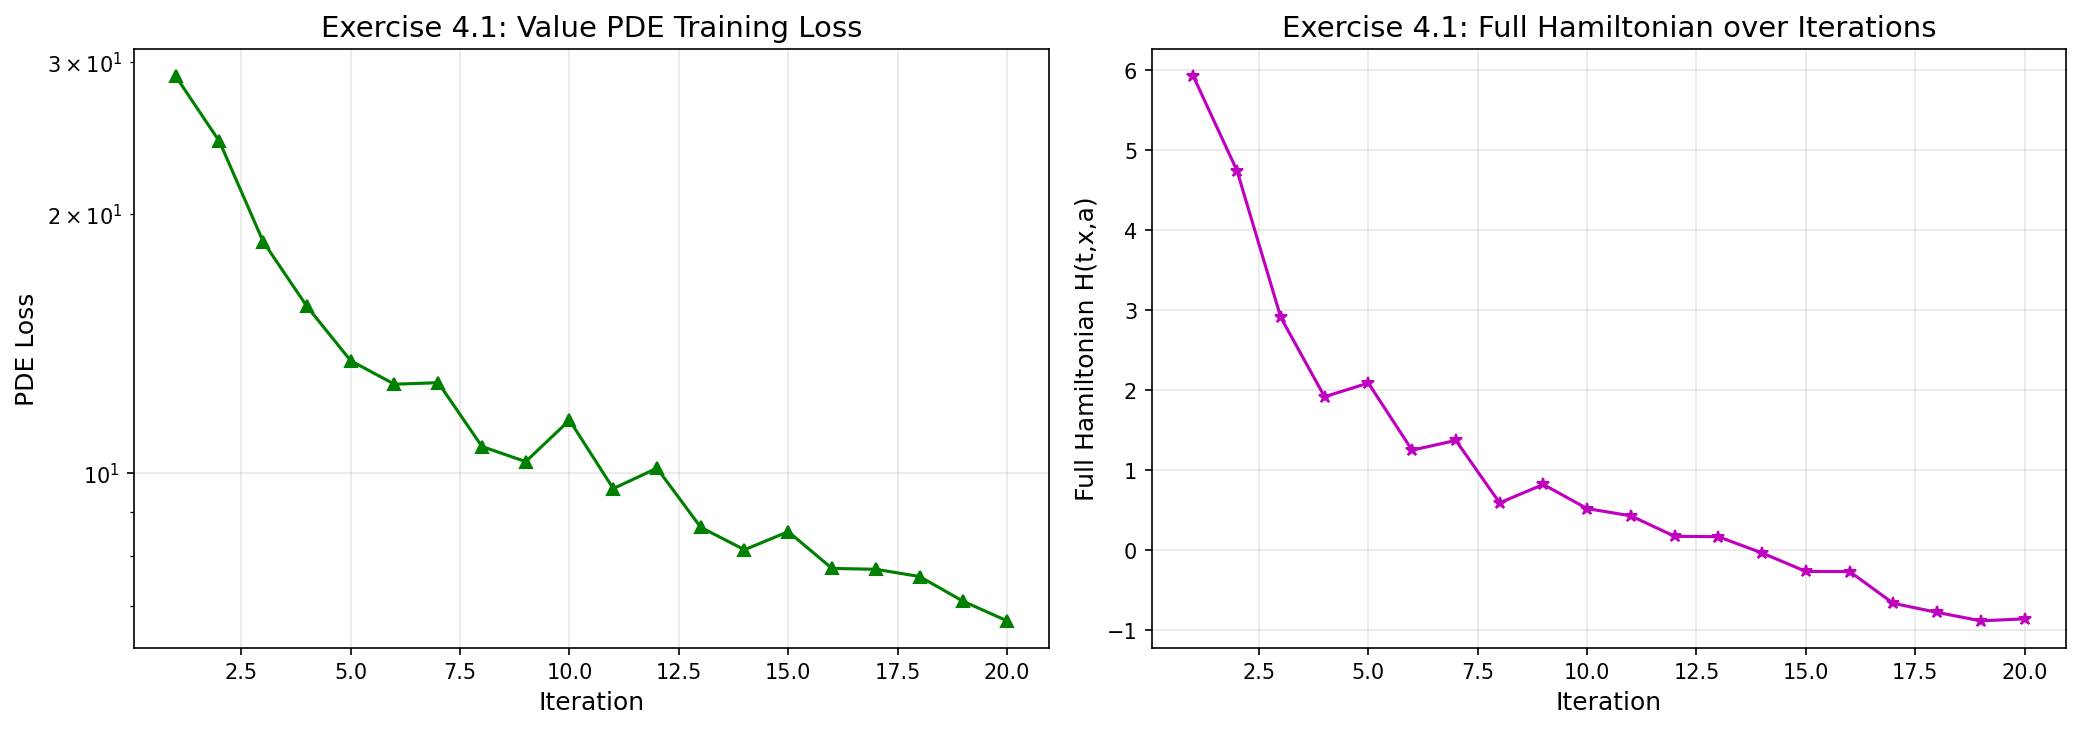
\includegraphics[width=0.7\linewidth]{figures/ex4_1_training_dynamics.png}
    \caption{Error of the PIA control $a(\cdot,\cdot;\theta_{\mathrm{act}})$
             relative to the optimal Riccati control across PIA iterations.}
    \label{fig:ex4.1_training}
\end{figure}

\begin{itemize}
\item \textbf{Value PDE Training Loss:} The residual loss decreases sequentially across iterations (e.g., from $\sim 20$ to $5$). This improvement occurs because the optimal value function becomes progressively smoother and easier to approximate as the control policy improves, and because the network retains learned features (warm-starting) between outer iterations.
\item \textbf{Hamiltonian Minimisation:} The Hamiltonian decreases steadily (becoming more negative, e.g., from $-5$ to $-10$). This confirms that each policy improvement step successfully finds a control output $a(t,x;\theta_{act})$ that directly reduces the instantaneous cost and directional derivative combination. The stabilisation in later iterations indicates convergence toward the theoretical optimum, where further minimisation yields diminishing returns.
\end{itemize}

% ============================================================
\section{Conclusion}
\label{sec:conclusion}

% TODO: brief summary of what was achieved and any limitations observed.
[Summarise your key findings: accuracy of the Riccati solver, the supervised
learning baselines, the DGM PDE solver, and the full PIA loop. Note any limitations
or areas for improvement.]

% ============================================================
\appendix
\section{Code Structure}
\label{app:code}

The full code is available at \url{https://github.com/YOUR_USERNAME/YOUR_REPO}.
A \texttt{README.md} at the root of the repository describes how to reproduce
all figures in this report.

% Brief description of key files/modules (optional but helpful):
% \begin{itemize}
%     \item \texttt{lqr.py} -- LQRSolver class (Exercises 1.1--1.2)
%     \item \texttt{networks.py} -- Net\_DGM and FFN architectures
%     \item \texttt{supervised.py} -- Exercises 2.1--2.2
%     \item \texttt{dgm.py} -- Deep Galerkin solver (Exercise 3.1)
%     \item \texttt{pia.py} -- Policy iteration (Exercise 4.1)
%     \item \texttt{assignment.ipynb} -- Jupyter notebook reproducing all plots
% \end{itemize}

\end{document}